% compile with: pdflatex -shell-escape filename.tex
\documentclass[crop,tikz,convert=pdf2svg]{standalone}
\usepackage{tikz}
\usetikzlibrary{backgrounds}
\usetikzlibrary{matrix}
\usetikzlibrary{patterns}

\tikzset{
  row 1/.style={
    color=black!50,
    font=\small,
  },
  column 1/.style={
    color=black!50,
    font=\small,
  },
}

\begin{document}

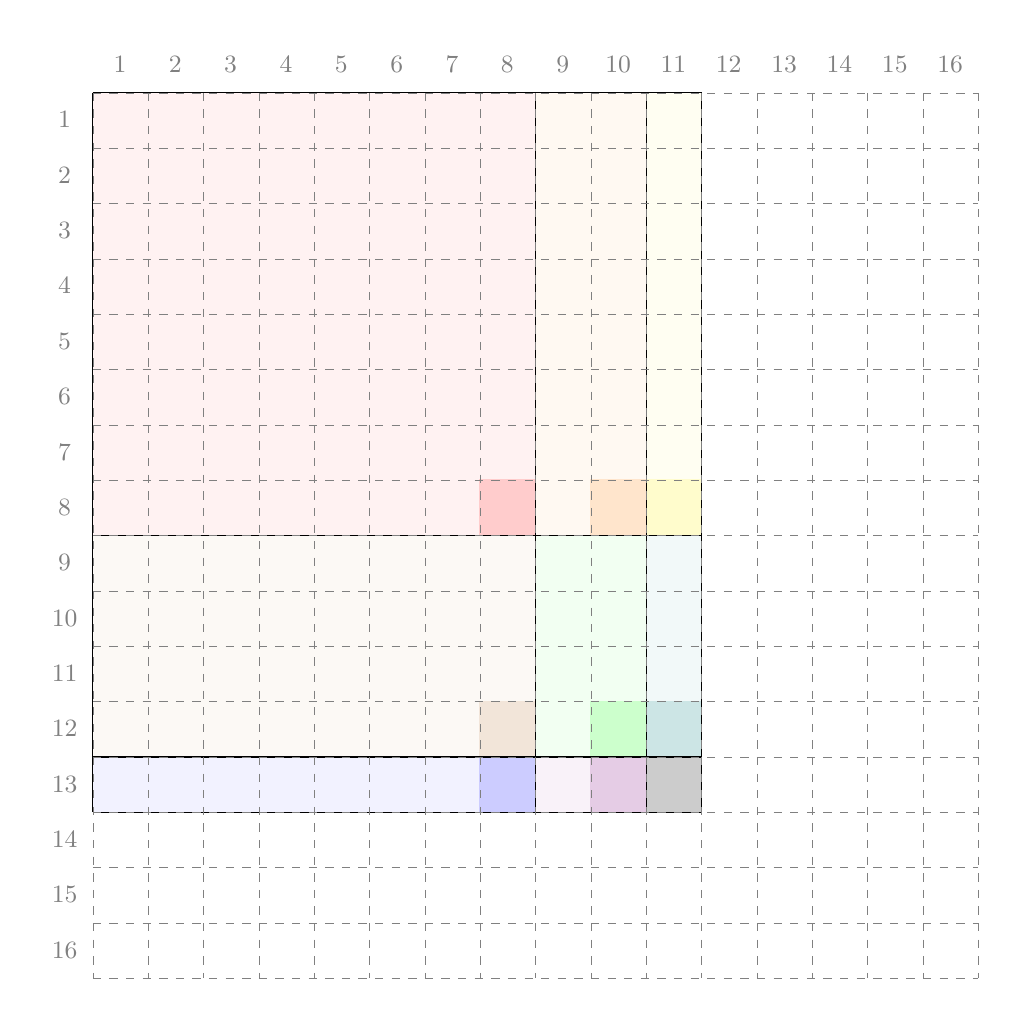
\begin{tikzpicture}

  \matrix (mat) at (2, 0) [
    matrix of nodes,
    nodes={anchor=center, minimum size=20pt},
  ] {
    \ & 1 & 2 & 3 & 4 & 5 & 6 & 7 & 8 & 9 & 10 & 11 & 12 & 13 & 14 & 15 & 16\\
    1 & \  & \  & \  & \  & \  & \  & \  & \  & \  & \  & \  & \  & \  & \  & \  & \ \\
    2 & \  & \  & \  & \  & \  & \  & \  & \  & \  & \  & \  & \  & \  & \  & \  & \ \\
    3 & \  & \  & \  & \  & \  & \  & \  & \  & \  & \  & \  & \  & \  & \  & \  & \ \\
    4 & \  & \  & \  & \  & \  & \  & \  & \  & \  & \  & \  & \  & \  & \  & \  & \ \\
    5 & \  & \  & \  & \  & \  & \  & \  & \  & \  & \  & \  & \  & \  & \  & \  & \ \\
    6 & \  & \  & \  & \  & \  & \  & \  & \  & \  & \  & \  & \  & \  & \  & \  & \ \\
    7 & \  & \  & \  & \  & \  & \  & \  & \  & \  & \  & \  & \  & \  & \  & \  & \ \\
    8 & \  & \  & \  & \  & \  & \  & \  & \  & \  & \  & \  & \  & \  & \  & \  & \ \\
    9 & \  & \  & \  & \  & \  & \  & \  & \  & \  & \  & \  & \  & \  & \  & \  & \ \\
    10 & \  & \  & \  & \  & \  & \  & \  & \  & \  & \  & \  & \  & \  & \  & \  & \ \\
    11 & \  & \  & \  & \  & \  & \  & \  & \  & \  & \  & \  & \  & \  & \  & \  & \ \\
    12 & \  & \  & \  & \  & \  & \  & \  & \  & \  & \  & \  & \  & \  & \  & \  & \ \\
    13 & \  & \  & \  & \  & \  & \  & \  & \  & \  & \  & \  & \  & \  & \  & \  & \ \\
    14 & \  & \  & \  & \  & \  & \  & \  & \  & \  & \  & \  & \  & \  & \  & \  & \ \\
    15 & \  & \  & \  & \  & \  & \  & \  & \  & \  & \  & \  & \  & \  & \  & \  & \ \\
    16 & \  & \  & \  & \  & \  & \  & \  & \  & \  & \  & \  & \  & \  & \  & \  & \ \\
  };

  \fill[black!20] (mat-14-12.north west) rectangle (mat-14-12.south east);

  \fill[violet!05] (mat-14-10.north west) rectangle (mat-14-10.south east);
  \fill[fill=violet!20] (mat-14-11.north west) rectangle (mat-14-11.south east);

  \fill[blue!05] (mat-14-2.north west) rectangle (mat-14-9.south east);
  \fill[fill=blue!20] (mat-14-9.north west) rectangle (mat-14-9.south east);

  \fill[teal!05] (mat-10-12.north west) rectangle (mat-13-12.south east);
  \fill[fill=teal!20] (mat-13-12.north west) rectangle (mat-13-12.south east);

  \fill[green!05] (mat-10-10.north west) rectangle (mat-13-11.south east);
  \fill[fill=green!20] (mat-13-11.north west) rectangle (mat-13-11.south east);

  \fill[brown!05] (mat-10-2.north west) rectangle (mat-13-9.south east);
  \fill[fill=brown!20] (mat-13-9.north west) rectangle (mat-13-9.south east);

  \fill[yellow!05] (mat-2-12.north west) rectangle (mat-9-12.south east);
  \fill[fill=yellow!20] (mat-9-12.north west) rectangle (mat-9-12.south east);

  \fill[orange!05] (mat-2-10.north west) rectangle (mat-9-11.south east);
  \fill[fill=orange!20] (mat-9-11.north west) rectangle (mat-9-11.south east);

  \fill[red!05] (mat-2-2.north west) rectangle (mat-9-9.south east);
  \fill[red!20] (mat-9-9.north west) rectangle (mat-9-9.south east);

  \draw (mat-1-1.south east) -- (mat-1-12.south east);
  \draw (mat-9-1.south east) -- (mat-9-12.south east);
  \draw (mat-13-1.south east) -- (mat-13-12.south east);
  \draw (mat-14-1.south east) -- (mat-14-12.south east);

  \draw (mat-1-1.south east) -- (mat-14-1.south east);
  \draw (mat-1-9.south east) -- (mat-14-9.south east);
  \draw (mat-1-11.south east) -- (mat-14-11.south east);
  \draw (mat-1-12.south east) -- (mat-14-12.south east);

  \foreach \x in {1,...,17} {
    \draw [help lines, dashed] (mat-1-\x.south east) -- (mat-17-\x.south east);
    \draw [help lines, dashed] (mat-\x-1.south east) -- (mat-\x-17.south east);
  }
\end{tikzpicture}

\end{document}
